%% fig_factor.tex -- the reduction of the weakened criterion to the factor.
%% Top row: HT^2(X x X) as a Kuenneth stack, its middle summand meeting the
%% kernel in zero, carried by Orlov's isomorphism to HT^2 of the eightfold
%% X x Xhat with the 2n^2 classes preserving ch(E).  Bottom row: HT^2 of one
%% factor X, three slabs with heights proportional to the dimensions 16, 6, 6
%% at n = 4, and inside them the n^2 = 16 classes: the polarised deformations
%% Sym^2 in H^1(T) and the Poisson directions, each compensated by a class in
%% H^{0,2}; and the two conditions the evaluation map imposes on them, one
%% closed and one open.
\documentclass[tikz,border=9pt]{standalone}
\usepackage{amsmath,amssymb}
\usetikzlibrary{arrows.meta,calc,backgrounds,positioning,decorations.pathreplacing}
%% palette.tex -- shared colour definitions for the figures
\definecolor{PInk}{RGB}{26,32,44}
\definecolor{PBlue}{RGB}{37,82,139}
\definecolor{PTeal}{RGB}{23,127,125}
\definecolor{POchre}{RGB}{193,138,44}
\definecolor{PClay}{RGB}{178,74,58}
\definecolor{PSlate}{RGB}{108,122,137}
\definecolor{PViolet}{RGB}{110,86,150}
\definecolor{WBlue}{RGB}{223,234,246}
\definecolor{WTeal}{RGB}{220,238,236}
\definecolor{WOchre}{RGB}{250,240,218}
\definecolor{WClay}{RGB}{247,229,224}
\definecolor{WSlate}{RGB}{238,241,244}
\definecolor{PMag}{RGB}{158,58,110}
\definecolor{PGrass}{RGB}{62,124,66}
\definecolor{PAmber}{RGB}{214,112,38}
\definecolor{PIndigo}{RGB}{58,64,140}
\definecolor{PRule}{RGB}{176,186,197}

%% shared macros so the standalone figures match the paper
\providecommand{\QQ}{\mathbb{Q}}
\providecommand{\ZZ}{\mathbb{Z}}
\providecommand{\RR}{\mathbb{R}}
\providecommand{\CC}{\mathbb{C}}
\providecommand{\PP}{\mathbb{P}}
\providecommand{\Kx}{K^{\times}}
\providecommand{\HW}{W}
\providecommand{\Nm}{\mathrm{N}}
\providecommand{\Hdg}{\mathrm{Hdg}}
\providecommand{\NS}{\mathrm{NS}}
\providecommand{\cA}{\mathcal{A}}
\providecommand{\cD}{\mathcal{D}}
\providecommand{\cF}{\mathcal{F}}
\providecommand{\cP}{\mathcal{P}}
\providecommand{\cO}{\mathcal{O}}
\providecommand{\cQ}{\mathcal{Q}}
\providecommand{\bbar}[1]{\overline{#1}}
\providecommand{\ch}{\operatorname{ch}}
\providecommand{\End}{\mathrm{End}}


\tikzset{obl/.style={x={(1cm,0cm)}, y={(0.50cm,0.36cm)}, z={(0cm,1cm)}}}

\newcommand{\slab}[7]{%
  \begin{scope}[obl]
    \fill[#7 top]   (#1,#2,#3+#6) -- (#1+#4,#2,#3+#6) -- (#1+#4,#2+#5,#3+#6) -- (#1,#2+#5,#3+#6) -- cycle;
    \fill[#7 front] (#1,#2,#3) -- (#1+#4,#2,#3) -- (#1+#4,#2,#3+#6) -- (#1,#2,#3+#6) -- cycle;
    \fill[#7 side]  (#1+#4,#2,#3) -- (#1+#4,#2+#5,#3) -- (#1+#4,#2+#5,#3+#6) -- (#1+#4,#2,#3+#6) -- cycle;
    \draw[#7 edge]  (#1,#2,#3) -- (#1+#4,#2,#3) -- (#1+#4,#2,#3+#6) -- (#1,#2,#3+#6) -- cycle;
    \draw[#7 edge]  (#1+#4,#2,#3) -- (#1+#4,#2+#5,#3) -- (#1+#4,#2+#5,#3+#6) -- (#1+#4,#2,#3+#6);
    \draw[#7 edge]  (#1,#2,#3+#6) -- (#1,#2+#5,#3+#6) -- (#1+#4,#2+#5,#3+#6);
  \end{scope}}

\tikzset{
  zz top/.style={fill=WBlue},   zz front/.style={fill=WBlue!80!PBlue!30},
  zz side/.style={fill=WBlue!60!PBlue!40}, zz edge/.style={draw=PBlue,line width=0.55pt},
  vv top/.style={fill=WClay},   vv front/.style={fill=WClay!80!PClay!30},
  vv side/.style={fill=WClay!60!PClay!40}, vv edge/.style={draw=PClay,line width=0.55pt},
  pp top/.style={fill=PViolet!14!white}, pp front/.style={fill=PViolet!26!white},
  pp side/.style={fill=PViolet!36!white}, pp edge/.style={draw=PViolet,line width=0.55pt},
  ker top/.style={fill=WTeal},  ker front/.style={fill=WTeal!80!PTeal!35},
  ker side/.style={fill=WTeal!60!PTeal!45}, ker edge/.style={draw=PTeal,line width=0.9pt},
  ext top/.style={fill=WSlate}, ext front/.style={fill=WSlate!85!PSlate!20},
  ext side/.style={fill=WSlate!70!PSlate!30}, ext edge/.style={draw=PSlate,line width=0.5pt},
  tt top/.style={fill=PClay!45!white}, tt front/.style={fill=PClay!55!white},
  tt side/.style={fill=PClay!65!white}, tt edge/.style={draw=PClay,line width=0.8pt},
}

\begin{document}
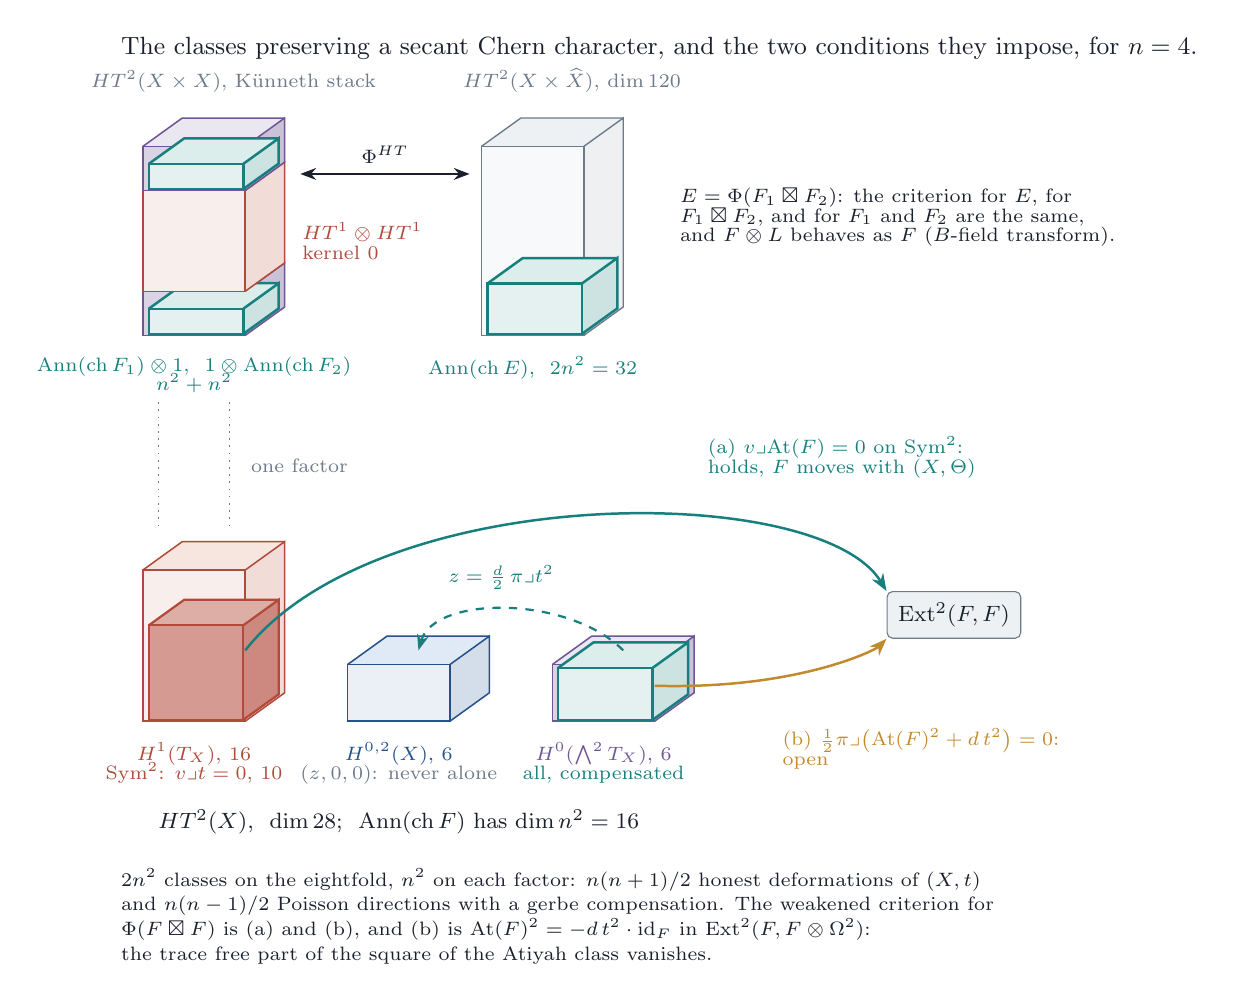
\begin{tikzpicture}[font=\small,text=PInk]

\node[anchor=west,font=\small,text=PInk] at (-0.4,8.55)
  {The classes preserving a secant Chern character, and the two conditions they impose, for $n=4$.};

%% =====================================================================
%% Top row: the product as a Kuenneth stack, and the eightfold, at 0.02 per
%% dimension
%% =====================================================================
\begin{scope}[shift={(0,4.9)}]
  \slab{0}{0}{0}{1.3}{1.0}{0.56}{pp}
  \slab{0.05}{0.05}{0}{1.2}{0.9}{0.32}{ker}
  \slab{0}{0}{0.56}{1.3}{1.0}{1.28}{vv}
  \slab{0}{0}{1.84}{1.3}{1.0}{0.56}{pp}
  \slab{0.05}{0.05}{1.84}{1.2}{0.9}{0.32}{ker}
  \slab{4.3}{0}{0}{1.3}{1.0}{2.4}{ext}
  \slab{4.35}{0.05}{0}{1.2}{0.9}{0.64}{ker}
  \begin{scope}[obl]
    \coordinate (Gt) at (0.65,1.0,2.4);
    \coordinate (Gb) at (0.65,0,0);
    \coordinate (Gm) at (1.3,0.0,1.2);
    \coordinate (Yt) at (4.95,1.0,2.4);
    \coordinate (Yb) at (4.95,0,0);
  \end{scope}
  \node[anchor=south,align=center,font=\scriptsize,text=PSlate] at ([yshift=2mm]Gt)
    {$HT^{2}(X\times X)$, K\"unneth stack};
  \node[anchor=north,align=center,font=\scriptsize,text=PTeal] at ([yshift=-1.5mm]Gb)
    {$\operatorname{Ann}(\ch F_{1})\otimes1$, \ $1\otimes\operatorname{Ann}(\ch F_{2})$\\[-1pt]$n^{2}+n^{2}$};
  \node[anchor=west,align=left,font=\scriptsize,text=PClay] at ([xshift=6mm]Gm)
    {$HT^{1}\otimes HT^{1}$\\[-1pt]kernel $0$};
  \node[anchor=south,align=center,font=\scriptsize,text=PSlate] at ([yshift=2mm]Yt)
    {$HT^{2}(X\times\widehat X)$, $\dim 120$};
  \node[anchor=north,align=center,font=\scriptsize,text=PTeal] at ([yshift=-1.5mm]Yb)
    {$\operatorname{Ann}(\ch E)$, \ $2n^{2}=32$};
  \draw[PInk,line width=0.8pt,{Stealth[length=2mm]}-{Stealth[length=2mm]}] (2.0,2.05) -- (4.15,2.05)
    node[midway,above,font=\scriptsize] {$\Phi^{HT}$};
  \node[anchor=west,align=left,font=\scriptsize,text=PInk] at (6.7,1.5)
    {$E=\Phi(F_{1}\boxtimes F_{2})$: the criterion for $E$, for\\[-1pt]
     $F_{1}\boxtimes F_{2}$, and for $F_{1}$ and $F_{2}$ are the same,\\[-1pt]
     and $F\otimes L$ behaves as $F$ ($B$-field transform).};
\end{scope}

% the zoom from the product to the factor: dotted lines down to the slab
\draw[PSlate,dotted,line width=0.6pt] (0.2,4.05) -- (0.2,2.45);
\draw[PSlate,dotted,line width=0.6pt] (1.1,4.05) -- (1.1,2.45);
\node[anchor=west,font=\scriptsize,text=PSlate] at (1.25,3.25) {one factor};

%% =====================================================================
%% Bottom row: one factor X, three slabs at 0.12 per dimension: 16, 6, 6
%% =====================================================================
% H^1(T), height 1.92, with Sym^2 (10) in front, height 1.2
\slab{0}{0}{0}{1.3}{1.0}{1.92}{vv}
\slab{0.05}{0.05}{0}{1.2}{0.9}{1.2}{tt}
% H^{0,2}, height 0.72, nothing of it alone in the kernel
\slab{2.6}{0}{0}{1.3}{1.0}{0.72}{zz}
% wedge^2 T, height 0.72, all of it in the kernel once compensated
\slab{5.2}{0}{0}{1.3}{1.0}{0.72}{pp}
\slab{5.25}{0.05}{0}{1.2}{0.9}{0.66}{ker}
\begin{scope}[obl]
  \coordinate (Vb) at (0.65,0,0);
  \coordinate (Vk) at (1.3,0.0,0.9);
  \coordinate (Zb) at (3.25,0,0);
  \coordinate (Zk) at (3.25,0.5,0.72);
  \coordinate (Pb) at (5.85,0,0);
  \coordinate (Pk) at (6.5,0.0,0.45);
  \coordinate (Pc) at (5.85,0.5,0.72);
\end{scope}
\node[anchor=north,align=center,font=\scriptsize,text=PClay] at ([yshift=-1.5mm]Vb)
  {$H^{1}(T_{X})$, $16$\\[-1pt]$\mathrm{Sym}^{2}$: $v\lrcorner t=0$, $10$};
\node[anchor=north,align=center,font=\scriptsize,text=PBlue] at ([yshift=-1.5mm]Zb)
  {$H^{0,2}(X)$, $6$\\[-1pt]{\color{PSlate}$(z,0,0)$: never alone}};
\node[anchor=north,align=center,font=\scriptsize,text=PViolet] at ([yshift=-1.5mm]Pb)
  {$H^{0}(\bigwedge^{2}T_{X})$, $6$\\[-1pt]{\color{PTeal}all, compensated}};
% the compensation: a dashed arrow from the bivectors to H^{0,2}
\draw[PTeal,dashed,line width=0.8pt,-{Stealth[length=2mm]}]
  (Pc) .. controls (5.4,1.6) and (3.7,1.6) .. (Zk);
\node[anchor=south,font=\scriptsize,text=PTeal] at (4.55,1.55)
  {$z=\tfrac d2\,\pi\lrcorner t^{2}$};
\node[anchor=north,font=\footnotesize,text=PInk] at (3.25,-1.0)
  {$HT^{2}(X)$, \ $\dim 28$; \ $\operatorname{Ann}(\ch F)$ has $\dim n^{2}=16$};

%% the two conditions
\node[draw=PSlate,fill=WSlate,rounded corners=2pt,inner sep=4pt,font=\footnotesize,align=center] (EX) at (10.3,1.35)
  {$\operatorname{Ext}^{2}(F,F)$};
\draw[PTeal,line width=0.9pt,-{Stealth[length=2.2mm]}]
  (Vk) .. controls (3.0,3.05) and (8.6,3.05) .. (EX.north west);
\draw[POchre,line width=0.9pt,-{Stealth[length=2.2mm]}]
  (Pk) .. controls (8.3,0.4) and (9.3,0.9) .. (EX.south west);
\node[anchor=west,align=left,font=\scriptsize,text=PTeal] at (7.05,3.35)
  {(a) $v\lrcorner\mathrm{At}(F)=0$ on $\mathrm{Sym}^{2}$:\\[-1pt]holds, $F$ moves with $(X,\Theta)$};
\node[anchor=west,align=left,font=\scriptsize,text=POchre] at (8.0,-0.35)
  {(b) $\tfrac12\pi\lrcorner\bigl(\mathrm{At}(F)^{2}+d\,t^{2}\bigr)=0$:\\[-1pt]open};

%% =====================================================================
%% Below: the summary lines
%% =====================================================================
\node[anchor=north west,align=left,font=\scriptsize,text=PInk] at (-0.4,-1.75)
  {$2n^{2}$ classes on the eightfold, $n^{2}$ on each factor: $n(n+1)/2$ honest deformations of $(X,t)$\\[1pt]
   and $n(n-1)/2$ Poisson directions with a gerbe compensation. The weakened criterion for\\[1pt]
   $\Phi(F\boxtimes F)$ is (a) and (b), and (b) is
   $\mathrm{At}(F)^{2}=-d\,t^{2}\cdot\mathrm{id}_{F}$ in $\operatorname{Ext}^{2}(F,F\otimes\Omega^{2})$:\\[1pt]
   the trace free part of the square of the Atiyah class vanishes.};

\end{tikzpicture}
\end{document}
